\documentclass[twocolumn,a4paper]{article}
\usepackage{graphicx, wrapfig}
\begin{document}
\title{exponential-function}
\author{Lasse Schwaner Arndt}
\maketitle
\begin{abstract}
	an abstract that grabs your attention and describes the report
\end{abstract}

\section{Introduction}
The exponential function is a mathematical Function 
denoted by $f(x)=\exp(x)$ or $e^x$ (where the argument $x$ 
is written as an exponentiation). It can be defined in 
Characterizations of the exponential function several equivalent ways. 
Its ubiquitous occurrence in pure mathematics and applied mathematics 
led mathematician Walter Rudin to opine that the exponential function is 
"the most important function in mathematics"
Its value at $1$, $e = \exp(1)$ is a mathematical constant
called Euler's number. \\

\section{The Func if funky}
The exponential function is defined by the power series:
\begin{equation}\label{eq-pwr}
	\exp x := \sum_{k = 0}^{\infty} \frac{x^k}{k!} = 1 + x + \frac{x^2}{2} + \frac{x^3}{6} + \frac{x^4}{24} + \cdots
\end{equation}

an approximation of which can be implemented in C\# by the expression:
\begin{figure}[ht!]
	\begin{verbatim}
	static double ex(double x){
		if(x<0)return 1/ex(-x);
		if(x>1.0/8)return Pow(ex(x/2),2); 
		return 1+x*(1+x/2*(1+x/3*(1+x/4*(1+x/5*
		(1+x/6*(1+x/7*(1+x/8*(1+x/9*(1+x/10)))))))));
		}
	\end{verbatim}
\end{figure}

Which obviously converges with the above expression when including an adequate number of fractions. The above approximation can be considered exact at the 32bit depth provided by the C\# doubles. This code works well as it uses only basic mathematic operators (division, multipliction) which can be done in the stack. As such it is both fast and accurate.
\begin{figure}[h!]\label{fig:exp}
	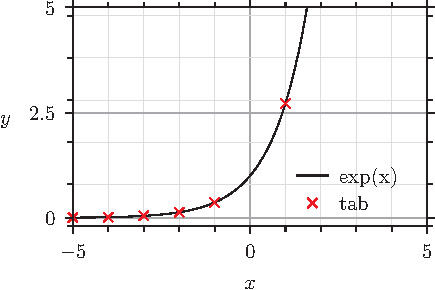
\includegraphics[width=\linewidth]{ex_pyx.pdf}
	\caption{depiction of the exponential function in range (-5,5)}
\end{figure}



\end{document}
